\documentclass[crop=false]{standalone}
\usepackage[utf8]{inputenc}
\usepackage{amsmath}
\usepackage[dvipsnames]{xcolor}
\usepackage{pdfpages}
\usepackage{enumerate}
\usepackage{amssymb}
\usepackage[framemethod=default]{mdframed}
\usepackage[nomarginpar,left=2cm,right=2cm,top = 2cm, bottom = 2cm]{geometry}

\renewcommand{\thesubsection}{\thesection.\alph{subsection}}
\renewcommand{\thesubsubsection}{\thesection.\alph{subsection}.\roman{subsubsection}}

\mdfdefinestyle{theoremstyle}{%
linecolor=black,linewidth=.3pt,%
frametitlerule=true,%
frametitlebackgroundcolor=blue!5,
innertopmargin=\topskip,nobreak=true,
}

\mdfdefinestyle{style2}{frametitle={},%
             linewidth=.3pt,topline=true,backgroundcolor=blue!3!green!8!}

\mdtheorem[style=theoremstyle]{task}{Angabe}

\newmdenv[style = style2,title=false]{solution}

\begin{document}
\begin{task}[Stabilität und Linearisierung]
Betrachten Sie das System
\[ 
\begin{aligned} \dot{x}_{1} &=-\alpha x_{1}-x_{1} x_{2} \\ \dot{x}_{2} &=\beta x_{1}^{2} \end{aligned}
 \]
 mit $\alpha, \beta>0$.
 \begin{enumerate}[i]
     \item Zeigen Sie die Stabilität der Ruhelage $\mathbf{x}_{s}=\mathbf{0}$ anhand der Lyapunovfunktion
     \[ 
V\left(x_{1}, x_{2}\right)=\frac{1}{2} x_{1}^{2}+\frac{1}{2 \beta} x_{2}^{2}
 \]
 \begin{solution}
    \[\dot{V} = \nabla V(\vec{x}) \cdot f(\vec{x}) = \nabla \left( \frac{1}{2} x_{1}^{2}+\frac{1}{2 \beta} x_{2}^{2} \right) \cdot f(\vec{x})\]
    \[\dot{V} = \begin{pmatrix}
    x_1 & \frac{x_2}{\beta}
    \end{pmatrix}
    \begin{pmatrix}
    -\alpha x_1 - x_1 x_2 \\
    \end{pmatrix}
    = - x_1^2 \alpha - x_1^2 x_2 + x_1^2 x_2
    = -x_1^2 \alpha
    \]
    Die orbitale Ableitung der Ljapunovfunktion ist nicht negativ definit, damit kann keine asymptotische Stabilität gezeigt werden. Die Ljapunovfunktion ist jedoch positiv definit und somit ist die Ruhelage stabil.
    \end{solution}
 \item Bestimmen Sie die Menge $S=\left\{\left(x_{1}, x_{2}\right) \in \mathbb{R}^{2} | \dot{V}\left(x_{1}, x_{2}\right)=0\right\}$ und skizzieren Sie diese in der $\left(x_{1}, x_{2}\right)$-Ebene.
 \begin{solution}
    \[\dot{V}\left(x_{1}, x_{2}\right)=-x_1^2 \alpha\]
    $\dot{V}$ ist genau dann $0$, wenn $x_1$ $0$ ist, die Funktion ist unabhängig von $x_2$. Trajektorien für $\alpha = \beta =  0$ geplottet. 
    
        {\centering
        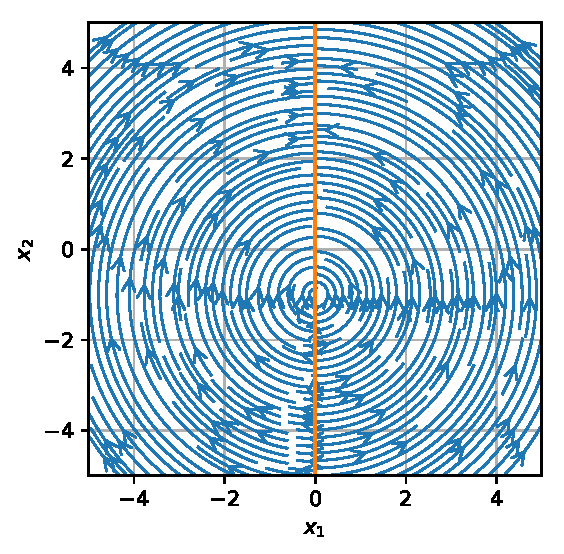
\includegraphics[width = 5cm]{LaSalle2017.pdf}
        \par}
    \end{solution}
\item Treffen Sie eine Stabilitätsaussage mit Hilfe des Invarianzprinzips von LaSalle. \emph{Begründung!}
\begin{solution}
    Es existieren Trajektorieren die sich vollständig in der invarianten Menge befinden, die Ruhelage ist nicht asymptotisch stabil.
    \end{solution}
 \end{enumerate}
\end{task}
\end{document}